\documentclass[11pt,a4paper]{article}
\usepackage[utf8]{inputenc}\usepackage[T1]{fontenc}\usepackage[spanish]{babel}\usepackage{lmodern}
\usepackage[a4paper,margin=2.2cm]{geometry}\usepackage{graphicx,booktabs,longtable,tabularx,array,xcolor,hyperref,fancyhdr,microtype}
\definecolor{Ink}{HTML}{10272F}\definecolor{Teal}{HTML}{18A999}\definecolor{Blue}{HTML}{2F6BFF}\definecolor{Gold}{HTML}{F2B134}\definecolor{Red}{HTML}{D85C5C}\definecolor{Paper}{HTML}{F5F7F5}\definecolor{Muted}{HTML}{61747B}
\hypersetup{colorlinks=true,linkcolor=Blue,urlcolor=Blue}\graphicspath{{../../presentacion/assets/}}
\pagestyle{fancy}\fancyhf{}\setlength{\headheight}{14pt}\lhead{Kaleido FlowTwin}\rhead{Phys-JEPA core -- claim\_eligible público}\cfoot{\thepage}
\newcommand{\claimbox}[1]{\begin{center}\fcolorbox{Gold}{Gold!18}{\parbox{.92\linewidth}{\textbf{#1}}}\end{center}}
\title{\textbf{Kaleido FlowTwin}\\Informe técnico y ejecutivo del MVP}\author{EVOCON Solutions -- Álvaro Schwiedop Souto}\date{2026-07-17}
\begin{document}\maketitle
\claimbox{Estado mixto y acotado: el core Phys-JEPA limpio es \texttt{claim\_eligible} sobre NOAA AIS público; ETA/OCEL históricos son \texttt{smoke\_only}. El gate completo y Kaleido siguen cerrados. No se demuestra ROI, causalidad ni despliegue.}
\section*{Resumen ejecutivo}
Se implementó y ejecutó un \textbf{Port Call Deviation Twin} read-only para Shipping Board/Freight Intelligence. El sistema predice estado físico a 0,5/1/2 horas y combina un trajectory GBT fuerte con estado/futuros Phys-JEPA. El clean test usa 57 viajes futuros del 8 al 14 de febrero de 2025, congelados y hasheados antes de construir targets.

Trajectory GBT obtiene 2.635 km MAE. El híbrido individual, media de tres seeds, obtiene 2.587 $\pm$ 0.053 km y gana al raw GBT en 3/3 seeds. El ensemble de tres modelos obtiene \textbf{2.326 km}, mejora 11.72\%; bootstrap emparejado por viaje IC95\% 5.90--17.13\%, $P(\mathrm{mejora})=0.9995$. La AUPRC de desviación cambia 0.880 a 0.904.

El resultado no arrastra otros outputs. ETA con 10\% de viajes etiquetados cambia 1.133 a 1.127 h, solo 0.59\%, bajo el gate del 1\%. Delay AUPRC retrocede 0.619 a 0.606. Por ello el core trayectoria/desviación se conserva shadow, ETA permanece GBT-only y el head de delay se rechaza. El gate completo, producción y Kaleido permanecen cerrados.

Como baseline complementario, \textbf{Boosting ETA} obtiene 1.88 horas MAE en 85 viajes futuros del 1 al 7 de febrero, con IC95\% 1.70--2.08 y estado \texttt{smoke\_only}.

La mediana del error es 1.37 horas; 42.0\% de los puntos queda dentro de $\pm$1 hora, 60.6\% dentro de $\pm$2 y 87.3\% dentro de $\pm$4. Mejora 75.9\% a una ETA distancia/velocidad y 31.2\% a la mediana puerto-distancia. Pasa los seis gates predeclarados del nuevo holdout. La cobertura P90 es 94.5\%, pero su anchura media de 9.04 horas obliga a mostrar incertidumbre y abstención.

El segundo dataset, OCEL 2.0 Container Logistics, prueba contratos objeto-céntricos y revisiones de plan. El grafo correcto reduce el MAE de test de 88.17 a 86.64 horas, pero validación seleccionó la traza plana; el gate del grafo permanece cerrado. Este resultado se usa para process intelligence y como diagnóstico de I+D, no como claim predictivo.

Los antiguos Event-JEPA, T-JEPA, Var-JEPA, Action-JEPA, Warehouse y LaDe se mantienen para explicar invalidaciones, colapso y selección de caso. No se usan como demostrador comercial.

La recomendación es demostrar el core físico y ETA dentro de Shipping Board/Freight Intelligence, llevar process intelligence a Trace Port/TWINPORTS y ejecutar el mismo gate sobre un export Kaleido futuro. Ningún resultado público prueba precisión o valor para Kaleido.

\section{Hipótesis y encaje con Kaleido}
\textbf{Hipótesis principal.} Un estado Phys-JEPA preentrenado sin outcomes puede aportar dinámica multihorizonte a un GBT de trayectoria cuando las labels son escasas, sin sustituir los baselines que ganen ETA o riesgo.

Shipping Board y Freight Intelligence aportan la superficie natural para ETA y excepciones. Trace Port declara eventos, turnos, equipos, packing lists, incidencias, histórico y API; TWINPORTS desarrolla estado físico y espacial. FlowTwin no debe competir con ellos: debe consumir posiciones/eventos versionados y devolver salidas read-only dentro de los productos existentes.

\section{Datos, provenance y protocolo}
\noindent\begin{tabularx}{\linewidth}{@{}>{\bfseries}p{2.6cm}X@{}}\toprule
Dataset principal & NOAA MarineCadastre AIS 2025, desarrollo 1 enero--7 febrero y clean holdout 8--14 febrero \\
Dominio & Cargueros/petroleros en Nueva York, Houston, Los Ángeles y Nueva Orleans \\
Task & Estado físico y shortfall a 0,5/1/2 h; ETA como probe separado \\
Split & Futuro fijo por viaje: 341 / 83 / 57 viajes \\
Test & 8--14 febrero 2025; 750 muestras; viajes disjuntos \\
Hashes & prefijos \texttt{4f1c7bce92f6...}; métricas \texttt{99b4162f7b40...} \\
Dataset secundario & OCEL 2.0 Container Logistics, 1,966 contenedores y 12,184 prefijos \\
Selección & Arquitectura, regularizador, heads y umbral solo con desarrollo/validación; test no influyó \\
Seeds & 3 (11, 42, 73) \\
Claim state & \texttt{claim\_eligible} para core público; gate completo/Kaleido cerrado \\
\bottomrule\end{tabularx}

Los siete ficheros holdout (1.431.169.298 bytes) se descargaron como contenido opaco y sus hashes se versionaron antes de construir targets. El primer build falló cerrado por confundir el hash del input v2 con el output v3; se corrigió en un commit separado antes de abrir el holdout. El primer clean run no entrenó por faltar el extra PyTorch y no produjo métricas; el segundo ejecutó el protocolo congelado en worktree limpio, commit \texttt{cdae9b7}, \texttt{dirty=false}.

\section{Resultado principal: Port Call Deviation Twin}
\begin{center}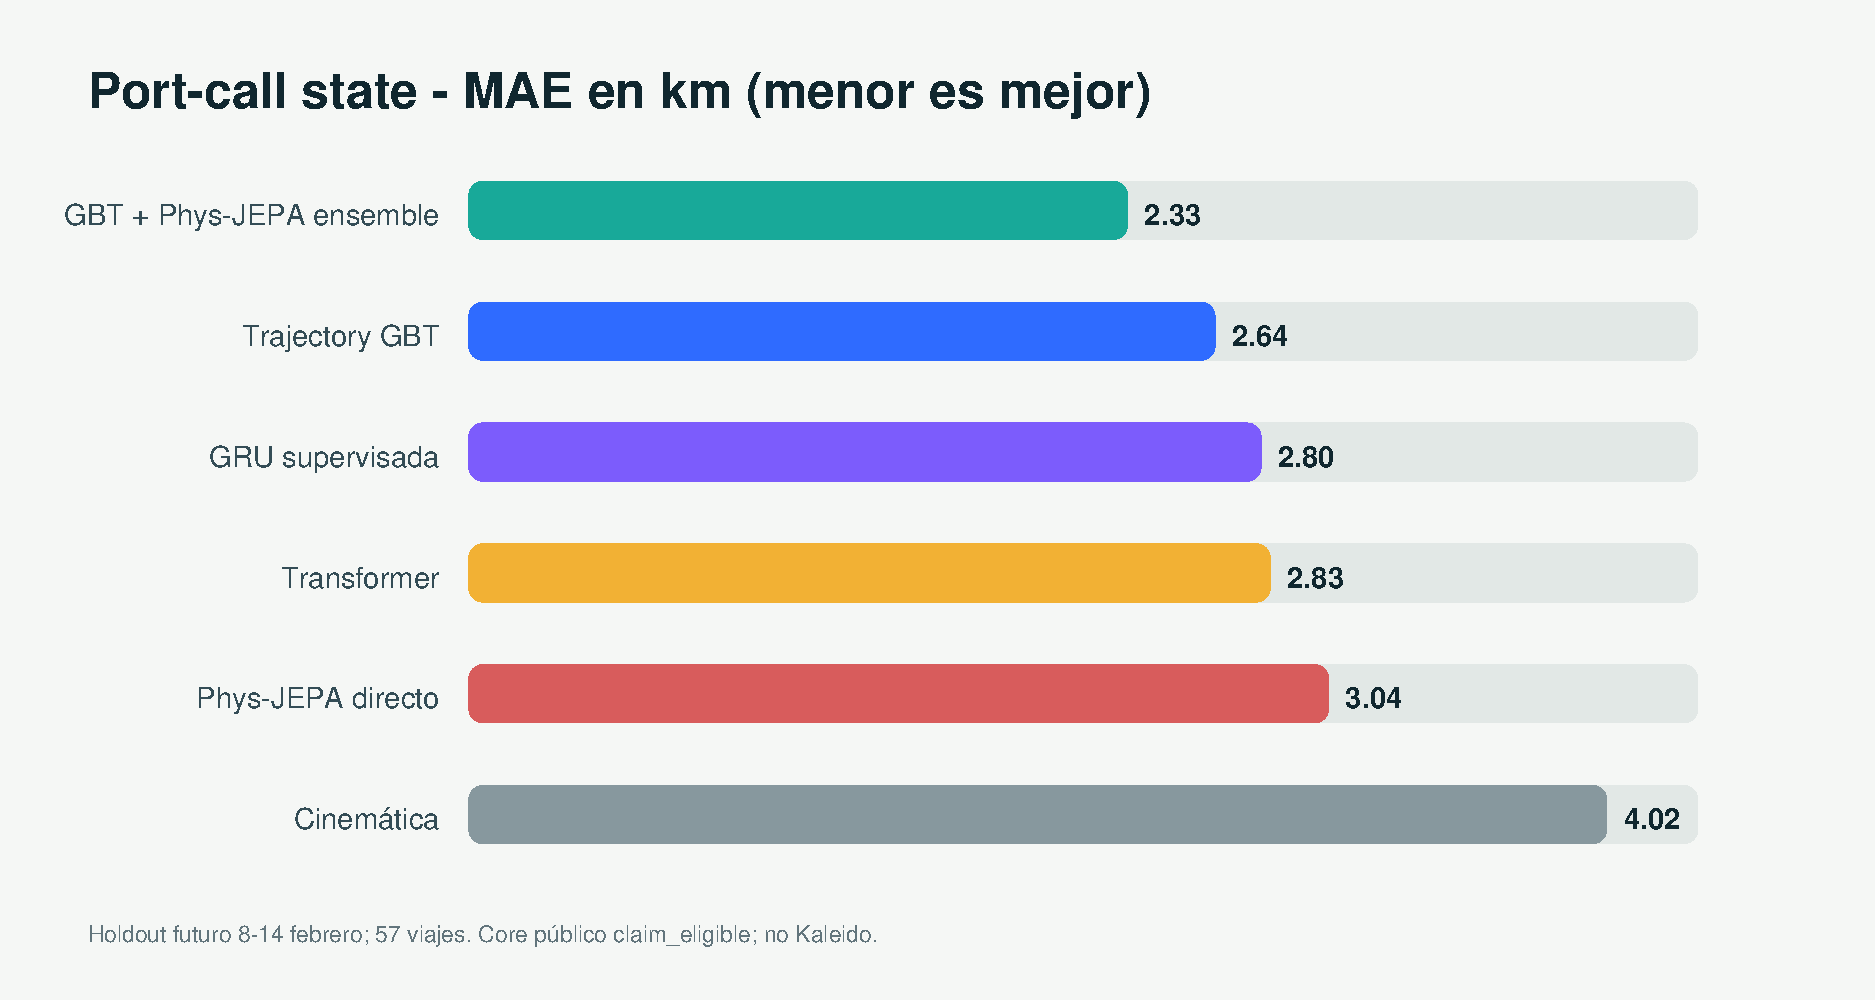
\includegraphics[width=.93\linewidth]{phys_jepa_clean.pdf}\end{center}
\begin{tabularx}{\linewidth}{XrrX}\toprule
Modelo & Seeds & MAE km & Lectura \\
\midrule
Cinemática de curso constante & -- & 4.018 & física sin aprendizaje \\
Trajectory GBT & 1 & 2.635 & floor supervisado \\
GRU / Transformer & 3 & 2.798 / 2.830 & baselines secuenciales \\
Phys-JEPA directo & 3 & 3.036 & decoder residual sin GBT \\
GBT + Phys-JEPA & 3 & 2.587 $\pm$ 0.053 & gana raw en 3/3 seeds \\
GBT + Phys-JEPA ensemble & 3 & \textbf{2.326} & candidato shadow \\
\bottomrule\end{tabularx}

El ensemble reduce MAE 11.72\%, con bootstrap emparejado por 57 viajes y 2.000 resamples: IC95\% 5.90--17.13\%, $P(\mathrm{mejora})=0.9995$. La media de seeds (2.587 km) mide estabilidad de entrenamiento; el ensemble (2.326 km) mide el candidato servido y su reducción de varianza. No deben confundirse.

La AUPRC de shortfall físico cambia 0.880 a 0.904. La cobertura conformal nominal 90\% alcanza 89.79\% con 12.00 km de ancho medio. El rango efectivo test es 11.42--12.46 y 0/3 representaciones colapsan.

\subsection{VISReg, SIGReg y otros controles de colapso}
\begin{center}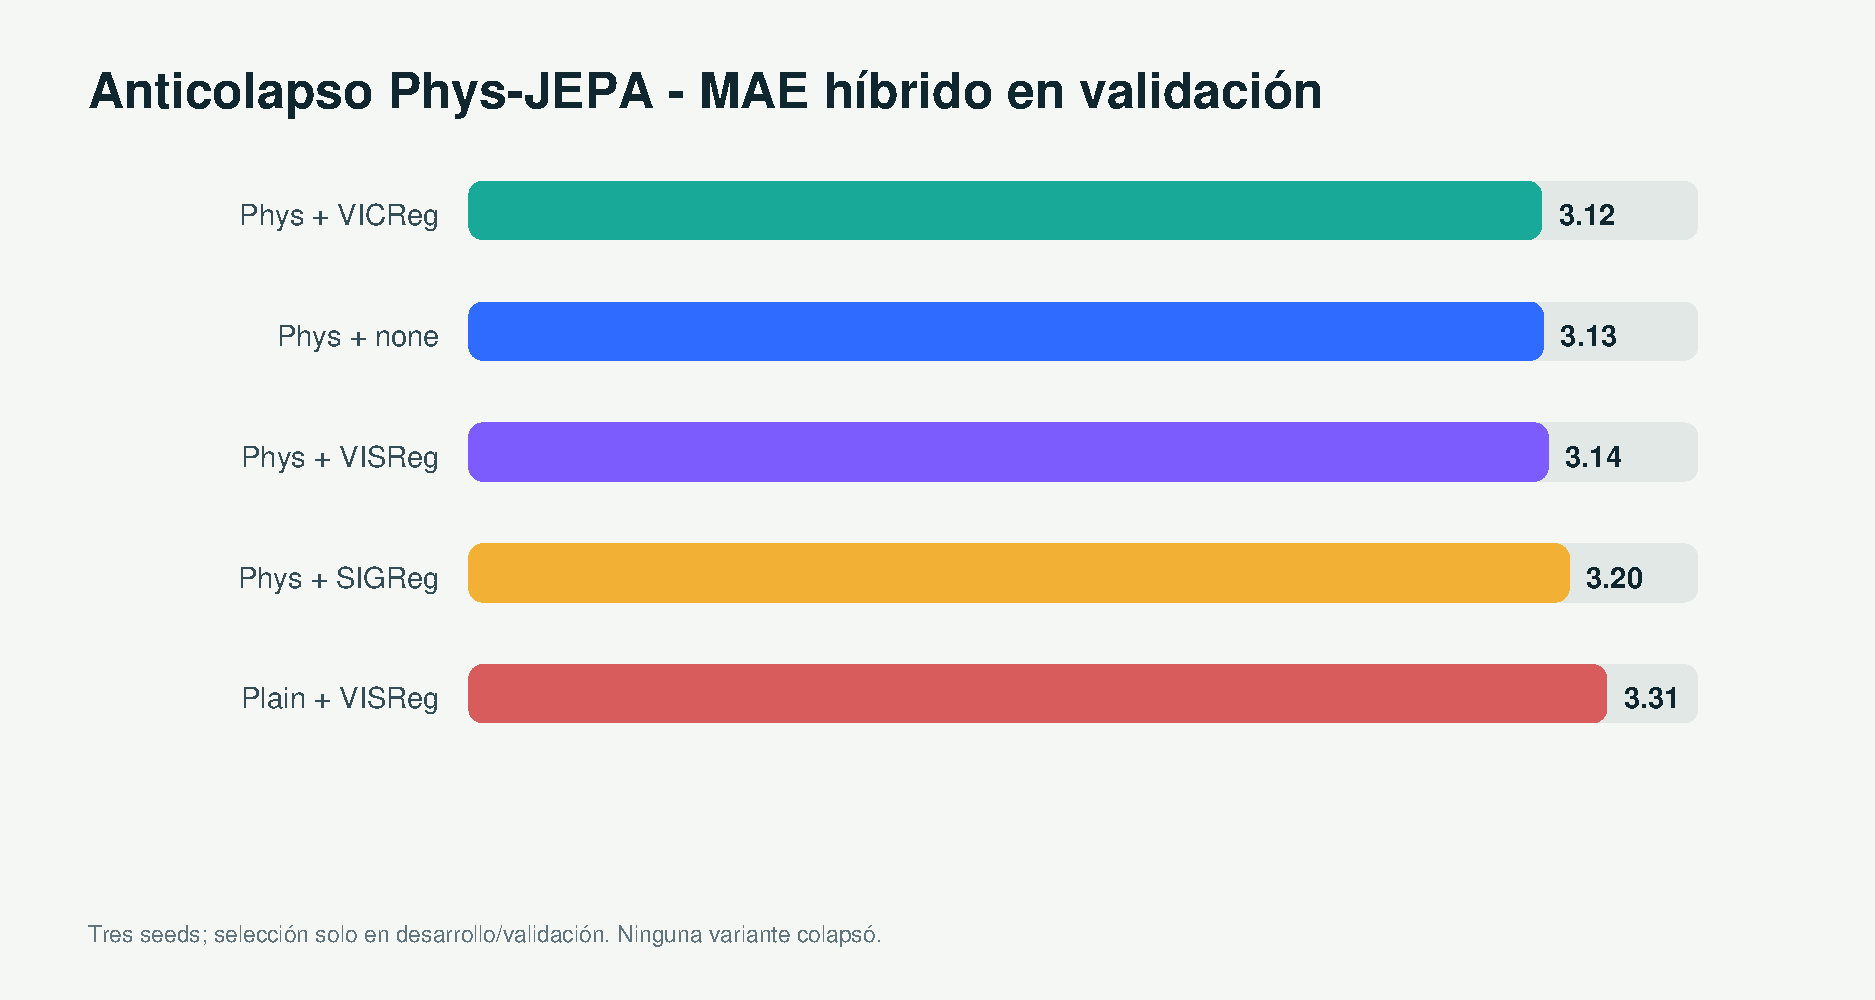
\includegraphics[width=.93\linewidth]{phys_jepa_regularizers.pdf}\end{center}
En desarrollo, el MAE híbrido de validación fue 3.124 km con VICReg, 3.129 sin regularizador, 3.143 con VISReg, 3.204 con SIGReg y 3.313 para JEPA sin física + VISReg. Ninguna variante colapsó. VICReg se seleccionó porque ganó el criterio predeclarado; el resultado sugiere que la inductive bias física aporta más que la diferencia entre losses anticolapso.

\subsection{Gate completo cerrado}
ETA escasa cambia 1.133 a 1.127 h (0.59\%), por debajo del mínimo del 1\%. Delay AUPRC cambia 0.619 a 0.606, una regresión. Por tanto el core físico pasa, pero el gate combinado y las promociones pública completa y Kaleido permanecen cerrados.

\section{Baseline complementario: ETA AIS}
\begin{center}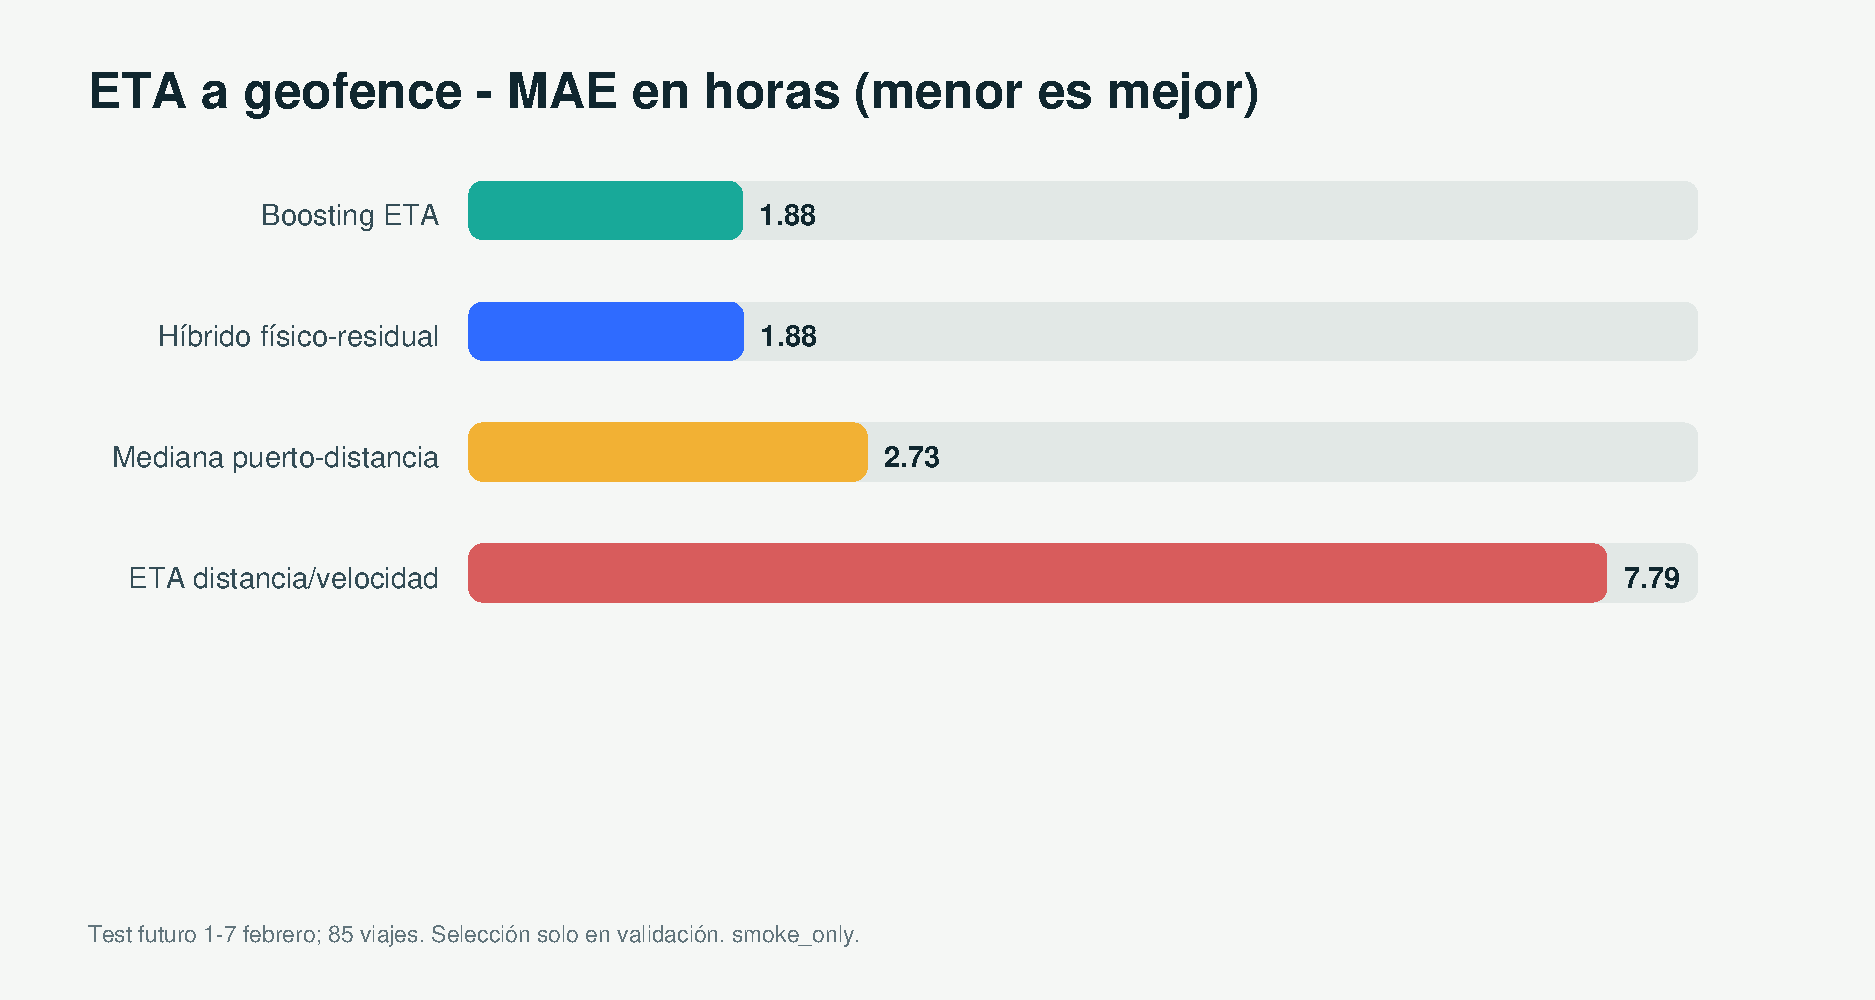
\includegraphics[width=.93\linewidth]{model_comparison.pdf}\end{center}
\begin{tabularx}{\linewidth}{Xrrrrl}\toprule
Modelo & MAE h & Mediana AE & $\pm$1 h & $\pm$2 h & Decisión \\
\midrule
Boosting ETA & 1.88 & 1.37 & 42.0\% & 60.6\% & seleccionado \\
Híbrido físico-residual & 1.88 & -- & -- & -- & segundo \\
Mediana puerto-distancia & 2.73 & -- & -- & -- & baseline histórico \\
ETA distancia/velocidad & 7.79 & -- & -- & -- & baseline físico \\
\bottomrule\end{tabularx}

Los seis gates predeclarados pasan: al menos 50 viajes, MAE máximo 2,5 h, extremo superior del IC95\% menor de 3 h, al menos 50\% dentro de $\pm$2 h y mejoras mínimas frente a ambos baselines. Por horizonte, el MAE es 1.96 h a 0--2 h, 1.49 h a 2--6 h y 2.13 h a 6--12 h.

\textbf{Límites.} 87.6\% de los prefijos de test pertenecen a Nueva Orleans. La cobertura P90 de 94.5\% usa intervalos de 9.04 h de anchura media. Las geofences son circulares inferidas y el dominio es EE. UU. El resultado habilita un demostrador de capacidad, no una promesa operativa para Kaleido.

\section{Process intelligence}
El loader OCEL público procesó 35,372 eventos, 13,882 objetos y 74,272 relaciones evento-objeto, con 47 variantes e integridad de grafo aprobada. Este bloque funciona sin entrenamiento y es el primer valor del piloto: variantes, tiempos de espera, rework, cuellos de botella, conformance y calidad temporal.

\section{Experimento histórico rechazado: Warehouse remaining time}
Este benchmark se conserva por auditabilidad y para estudiar JEPA, pero se retira de la demostración predictiva. Su escala absoluta e intervalo no resultan adecuados frente al nuevo ejemplo AIS.
\begin{tabularx}{\linewidth}{Xrrrrl}\toprule
Modelo & Seeds & MAE min & SD/IC & P90 & Decisión \\
\midrule
Boosting histórico & 1 & 734.51 & IC 697.99--771.49 & 90.02\% & referencia \\
Raw boosting rerun & 3 & 734.38 & SD 0.23 & -- & no servir \\
Raw + Var-JEPA & 3 & 738.98 & SD 0.60 & -- & rechazado \\
Temporal T-JEPA & 3 & 759.38 & SD 1.15 & -- & shadow I+D \\
Var-Event-JEPA & 3 & 760.41 & SD 6.25 & -- & shadow I+D \\
Event-JEPA frozen & 3 & 763.51 & SD 2.84 & 93.12\% & shadow I+D \\
ProcessTransformer & 3 & 809.54 & SD 17.89 & -- & no supera floor \\
\bottomrule\end{tabularx}

\subsection{Por qué los aproximadamente 700 minutos no son el demostrador}
El MAE histórico de 734.51 minutos equivale a 12.24 horas de error absoluto medio. La comparación relativa dentro del protocolo sigue siendo válida: mejora 6.9\% a la mediana global y 5.8\% a la mediana por actividad. Sin embargo, ganar por poco a baselines débiles no convierte la escala absoluta en una predicción presentable.

La lectura tampoco debe quedarse en la media. El error absoluto mediano de boosting es 363.98 minutos, frente a 353.15 de la mediana global; por tanto, la mejora de MAE procede sobre todo de reducir errores grandes, no de ganar en cada caso típico. El peor grupo, \texttt{S}, alcanza 1045.82 minutos. La cobertura P90 es 90.02\% con anchura media 2459.90 minutos, 41.00 horas. Ese intervalo amplio evidencia incertidumbre elevada y debe mostrarse.

La conclusión es de rechazo: este predictor no se sirve ni se usa como ejemplo comercial. Se mantiene como resultado negativo que motivó buscar una tarea más cercana a Shipping Board/Freight Intelligence. El benchmark AIS expresa error en horas, supera gates absolutos y compara contra una ETA física; aun así continúa en \texttt{smoke\_only}.

\subsection{Proxy de riesgo}
No existe plan versionado en el dataset, por lo que el target es duración larga por encima del P75 de training, no desviación material. AUPRC 0.567, ECE 0.223 y 33.97 falsas alertas por 100 operaciones son diagnósticos de desarrollo. No habilitan alerta portuaria ni claim de early warning.

\section{Event-JEPA y ablations}
\begin{center}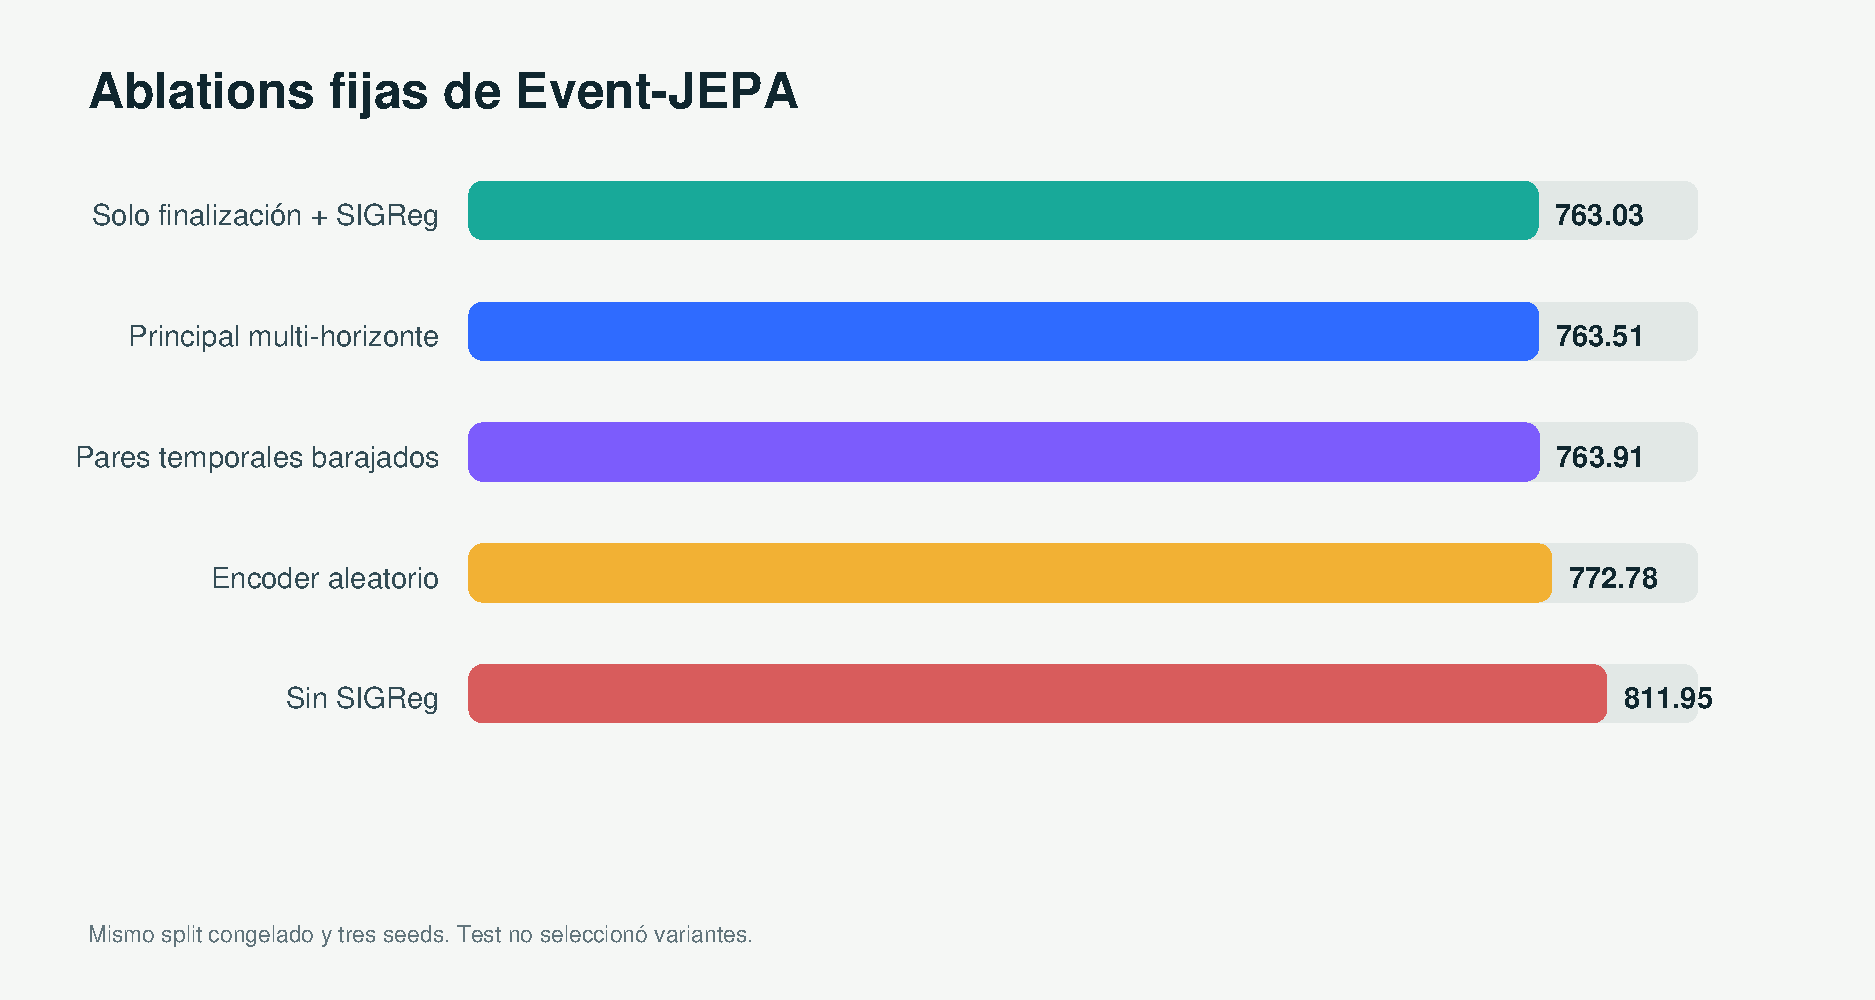
\includegraphics[width=.93\linewidth]{jepa_ablations.pdf}\end{center}
\begin{tabularx}{\linewidth}{lrrX}\toprule
Variante & MAE & SD & Lectura \\
\midrule
Main multi-horizon + SIGReg & 763.51 & 2.84 & referencia seleccionada en validación \\
Completion-only + SIGReg & 763.03 & 1.77 & multi-horizonte no aporta mejora \\
Shuffled temporal pairs & 763.91 & 2.15 & diferencia media 0.40; no consistente por seed \\
Random encoder, no JEPA & 772.78 & 2.67 & el objetivo JEPA aporta señal \\
Multi-horizon sin SIGReg & 811.95 & 13.90 & colapso; regularizador necesario \\
\bottomrule\end{tabularx}

La interpretación correcta no es ``JEPA gana''. Es: (1) hay valor de representación frente a encoder aleatorio; (2) SIGReg es necesario en el log; (3) no se ha validado ventaja multi-horizonte; (4) el emparejamiento temporal apenas cambia el downstream, por lo que aún no hay evidencia robusta de dinámica futura rica.

\section{Temporal T-JEPA, Var-JEPA y boosting híbrido}
Temporal T-JEPA corrige dos debilidades de la primera implementación: el target contiene solo el sufijo futuro y un teacher EMA con stop-gradient produce la representación objetivo. La regularización se eligió entre SiGReg, VISReg y token de registro usando validación. \texttt{multi\_visreg} obtiene 759.38 $\pm$ 1.15; completion-only obtiene 761.43 y el futuro barajado 762.91. El futuro correcto gana al barajado en 3/3 seeds, pero multi-horizonte no gana a completion-only en todas.

Var-Event-JEPA sustituye el punto latente determinista por distribuciones gaussianas de contexto, variable auxiliar y futuro. El ELBO combina reconstrucción, generación y términos KL. Obtiene 760.41 $\pm$ 6.25; la correlación Spearman media entre incertidumbre latente y error es 0.045, con dos seeds negativas. Esa incertidumbre es diagnóstica y no está calibrada en minutos.

El experimento híbrido entrena raw, raw+T-JEPA, raw+Var-JEPA y raw+ambos con el mismo split y tres seeds. Validación selecciona raw. Entre híbridos selecciona \texttt{raw\_var\_jepa}, que obtiene 738.98 $\pm$ 0.60, frente a 734.38 $\pm$ 0.23 de raw. La diferencia de 4.60 minutos cierra el gate de promoción.

\textbf{Lectura ELI5.} Boosting ve directamente reloj, progreso, actividad y espera. JEPA comprime una traza corta en un vector; en este log regular el resumen descarta detalle temporal y añade ruido. Esto no prueba que JEPA sea inferior en general: indica que todavía no gana su complejidad sin planes, objetos, contexto o acciones reales más ricos.

\section{Acciones sintéticas y world model}
Las actividades públicas no se relabelaron como acciones. Se generó un overlay separado con acciones timestamped, propensión, elegibilidad, coste y efecto estructural conocido. El boosting de recuperación v1 falló correct-vs-shuffled. El Action-Event-JEPA con SIGReg mejoró en media, pero no en cada seed y colapsó. La ablation condicional VISReg se activó porque había colapso en validación.

\begin{center}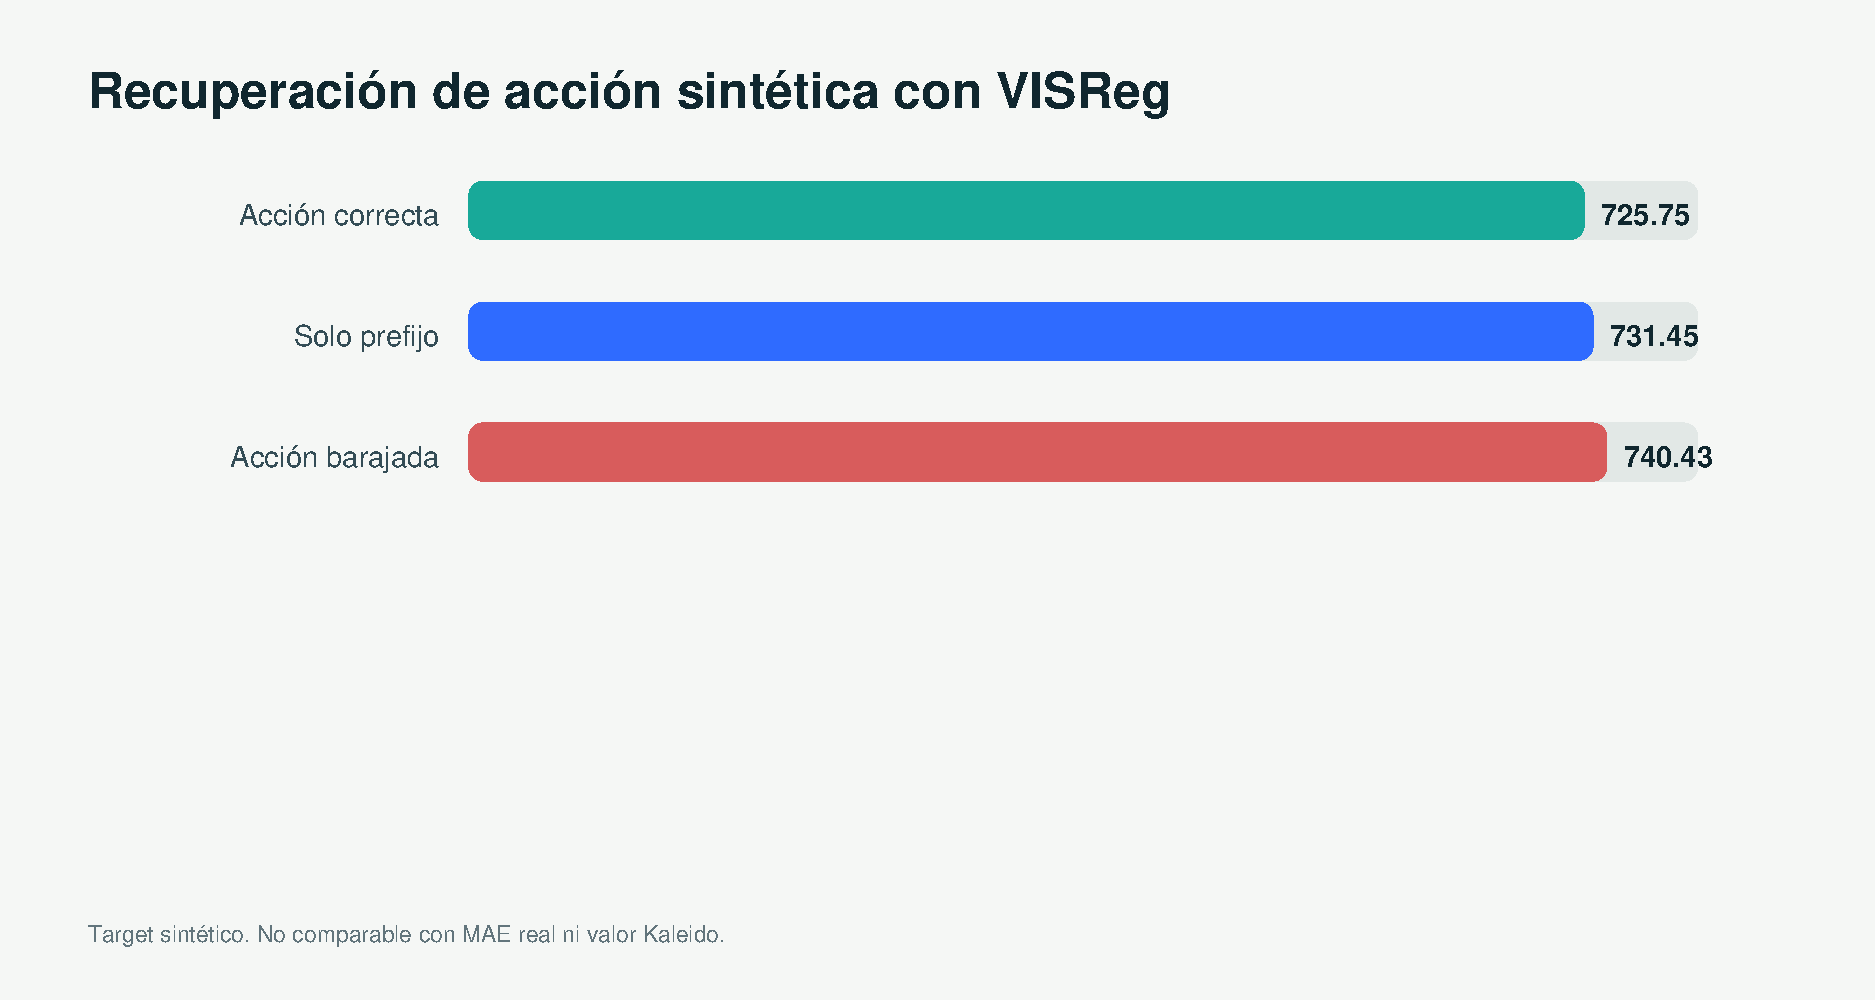
\includegraphics[width=.93\linewidth]{action_recovery.pdf}\end{center}
VISReg obtiene 725.75 $\pm$ 3.20 minutos con acción correcta frente a 740.43 con acción barajada y 731.45 con prefijo solo. Correct gana en 3/3 seeds y mejora 14.67 minutos de media frente a shuffled. Sin embargo, aunque el rango efectivo sube a 15.41--16.16, la desviación media por dimensión permanece 0.020--0.023, bajo el umbral. El resultado prueba recuperación de señal inyectada, no un world model operativo estable.

\section{Serving y producto recomendado}
La entrada demostrable es un Port Call Deviation Twin shadow embebible en Shipping Board o Freight Intelligence. Expone futuro físico 0,5/1/2 h, shortfall, AUPRC/score, latent surprise, intervalo conformal y procedencia. ETA continúa con su GBT separado. Trace Port/TWINPORTS reciben la excepción y process intelligence. Cada salida expone cutoff, geofence/plan visible, gate, confianza/abstención, razones y fuente. El sistema continúa read-only y los escenarios permanecen separados y etiquetados como simulación.

\section{Seguridad, límites y gates de piloto}
\begin{itemize}
\item conectores y API read-only; sin endpoints de escritura ni control de equipos;
\item seudonimización bajo control de Kaleido; fotos/notas fuera del primer modelo;
\item planes inmutables por \texttt{valid\_from}; censura explícita; split por operación;
\item umbrales en validación; reference model congelado; adaptación solo shadow con rollback;
\item GDPR, retención, roles y revisión de operador pendientes antes del piloto.
\end{itemize}

\claimbox{Lo que esto no demuestra: precisión o valor para Kaleido; generalización portuaria; desviación material; causalidad o contrafactuales; ROI, ahorro realizado, producción o despliegue exitoso.}

\section{Próximo paso falsable}
Sesión de 90 minutos para elegir una operación repetible, usuario/buyer, desviación material, acción disponible y coste de intervenir. Solicitar esquema y 3--5 operaciones pseudonimizadas para validar semántica; después un histórico suficiente con plan original y revisiones, outcomes y acciones timestamped. Ejecutar replay shadow 4--8 semanas con gates preacordados de cobertura, falsas alertas, lead time, peor grupo y utilidad del operador.

\section*{Cierre de tarea}
\textbf{Hipótesis:} Phys-JEPA puede aportar dinámica multihorizonte a un GBT fuerte sin sustituir los heads donde no gana.\\
\textbf{Cambios:} holdout futuro prehasheado, Phys-JEPA físico-residual, VISReg/SIGReg/VICReg/none, GBT/GRU/Transformer, bootstrap, conformal, API/dashboard e informes.\\
\textbf{Tests:} suites unitarias/integración/adversariales, lint y typing; hashes de los runs citados verificados al generar este documento.\\
\textbf{Evidencia:} core GBT + Phys-JEPA 2.635 a 2.326 km, IC95\% de mejora 5.90--17.13; AUPRC 0.880 a 0.904; gate completo cerrado por ETA/delay.\\
\textbf{Limitaciones:} AIS de EE. UU., 57 viajes, proxy físico e intervalo de 12.00 km; no hay datos Kaleido, outcomes materiales ni acciones reales.\\
\textbf{Siguiente paso falsable:} replay sobre export Kaleido congelado y revisión operativa.

\section*{Fuentes primarias y corporativas}
\begin{itemize}\small
\item \href{https://www.kaleidologistics.com/en/productos-ktech/trace-port/}{Kaleido Trace Port -- producto oficial}
\item \href{https://www.kaleidologistics.com/es/proyectos-financiados/el-proyecto-twinports-despega-en-el-puerto-de-vigo-comienzan-los-trabajos-para-crear-el-gemelo-digital-de-la-terminal-portuaria-de-kaleido/}{Kaleido TWINPORTS -- proyecto oficial}
\item \href{https://coast.noaa.gov/digitalcoast/tools/ais.html}{NOAA MarineCadastre AccessAIS -- fuente oficial}
\item \href{https://coast.noaa.gov/data/marinecadastre/ais/faq.pdf}{NOAA AIS FAQ -- cálculo de ETA y cobertura}
\item \href{https://doi.org/10.5281/zenodo.18373888}{OCEL 2.0 Container Logistics -- registro oficial}
\item \href{https://doi.org/10.6084/m9.figshare.29500898}{Warehouse Outbound Event Log -- DOI}
\item \href{https://arxiv.org/abs/2511.08544}{LeJEPA}; \href{https://arxiv.org/abs/2603.19312}{LeWorldModel}
\item \href{https://arxiv.org/abs/2606.02572}{VISReg}; \href{https://haiyuwu.github.io/visreg/}{proyecto oficial}
\item \href{https://arxiv.org/abs/2301.08243}{I-JEPA}; \href{https://arxiv.org/abs/2606.16076}{Phys-JEPA}; \href{https://arxiv.org/abs/2506.09985}{V-JEPA 2}
\item \href{https://arxiv.org/abs/2410.05016}{T-JEPA}; \href{https://arxiv.org/abs/2603.20111}{Var-JEPA}
\end{itemize}
\end{document}